\section{Track and Trail}

\subsection{Bounding box tracking}

In order to keep track of the same bounding box we add an algorithm to give each bounding box an ID by comparing their position.

\begin{figure}[H]
    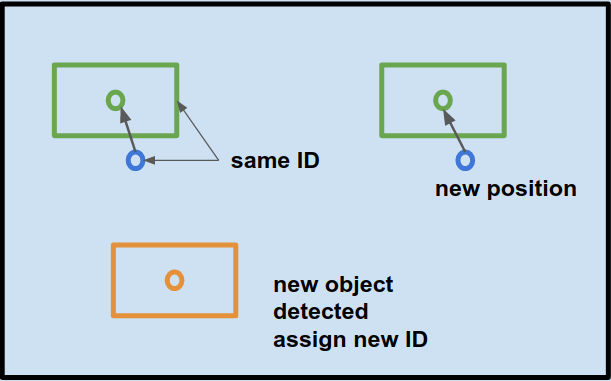
\includegraphics[width=1\columnwidth]{images/bbox.png}
    \centering
    \caption{bounding box id}
    \label{figure:bbox}
\end{figure}

\subsection{Tracking}

We use the bounding box of the target object as control signals. The height of the box indicate the distance between the target and boat. The position of the box indicates the orientation to the target. Then we use two PID controllers to control the distance and angle to keep track of the target.

\begin{figure}[H]
    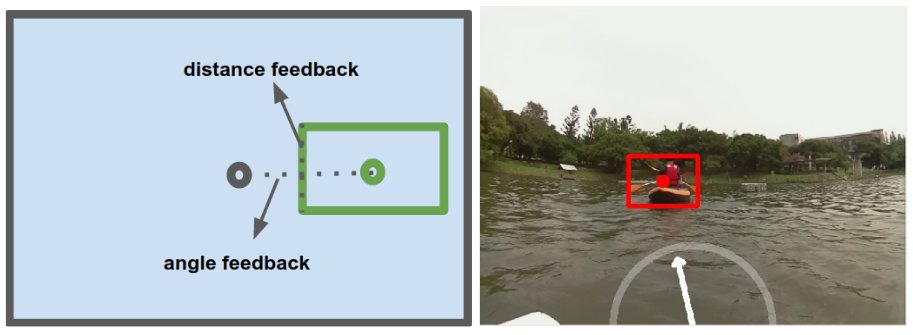
\includegraphics[width=1\columnwidth]{images/tracking.png}
    \centering
    \caption{tracking PID}
    \label{figure:tracking}
\end{figure}
